\section{Introduction}
% Introduction and research questions: What is the problem? Illustrate with an example. What is/are your research questions/contributions? 
\subsection{The Art Gallery Problem}

The Art Gallery Problem \cite{o1987art} is a central problem in computational geometry. It can be introduced as follows: given a simple polygon $P$ with $n$ vertices, we are interested in finding the minimum number of guards (points) that are able to see the whole polygon. A simple polygon is a polygon that has no holes. Thus, we can define the visibility of a point $g$ in the polygon $P \subset \mathbb R^2$. The point (guard) $g \in P$ sees another point $q \in P$ if the line segment $\overline{gq} \subseteq P$. The points that are visible from $g$ form the visibility polygon (region) $\mathit{Vis}(g)$. In the Art Gallery Problem, we are looking for a minimum size guard set $S$ that can see the whole polygon $P$.

Figure \ref{fig:art} displays an example of the Art Gallery Problem \cite{o1987art} with polygon $P$ guarded by 2 points ($|S| = 2$). The visibility region $\mathit{Vis}$ of each guard is marked with a different colour. For point $g \in S$, its visibility region $\mathit{Vis}(g)$ is emphasised with the pink contour. The vertex $r$ blocks part of the view of $g$. For this reason, it is called ``reflex'', because the angle it forms on the inside of the polygon is larger than $180^\circ$. Reflex vertices are only found in concave polygons, so convex polygons can be guarded by only one guard.

\begin{figure}[h!]
    \centering
    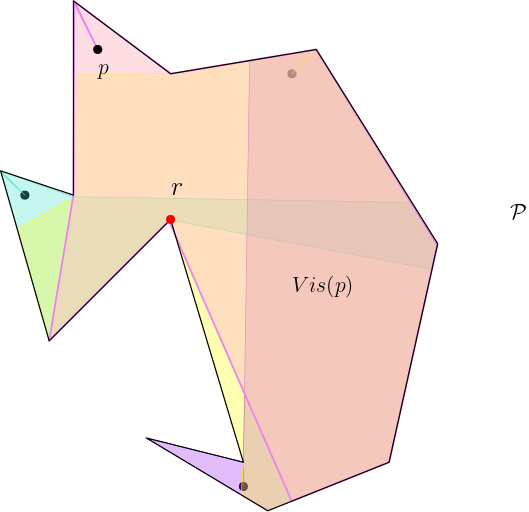
\includegraphics[width = 0.6\textwidth]{p.png}
    \caption{Example of an Art Gallery Problem instance with polygon $P$ guarded by 2 points. The visibility area $\mathit{Vis}(g)$ is emphasised in pink.}
    \label{fig:art}
\end{figure}

The Art Gallery Problem \cite{o1987art} is $\exists \mathbb R$-complete \cite{abrahamsen2021art}, which means it is even harder to solve than NP-complete problems. For this reason, approximation algorithms have been extensively used to address it (\cite{DBLP:journals/corr/BonnetM16b}, \cite{GHOSH2010718}, \cite{DBLP:journals/corr/abs-2007-06920}). Nonetheless, to the best of our knowledge there is no related work on approaching the Art Gallery Problem \cite{o1987art} using gradient descent. As such, we will approach the Art Gallery Problem \cite{o1987art} from a new perspective using gradient descent.

\newpage
\subsection{Gradient Descent}

Gradient descent is an iterative optimisation algorithm for finding the minimum of a continuous differentiable function. The core idea of gradient descent is to repeatedly move in the opposite direction of the gradient of the function at the current point using a specific step size (learning rate). High learning rates result in approaching a local optimum faster, but risk overshooting it. Conversely, small learning rates are more precise, with the compromise of a longer computation and convergence time.
When there is no more change in the gradient, then an optimum has been reached. Gradient descent does not guarantee that the found optimum is global. For this reason, it can remain stuck in local optima.

Figure \ref{fig:gradient_descent} illustrates an intuitive example of applying gradient descent. The optimisation function takes the shape of a curve. Starting from an arbitrary point on the curve, the goal is to reach the minimum of the function (the bottom of the curve). This is done by computing the gradient (derivative) of the function at the current point and moving in its opposite direction. In this case, the gradient would indicate going up the curve. In order to reach the minimum, the point has to move down the curve with the given step size. Continuing from the new point on the curve, the process is repeated until the minimum is reached.

\begin{figure}[h!]
    \centering
    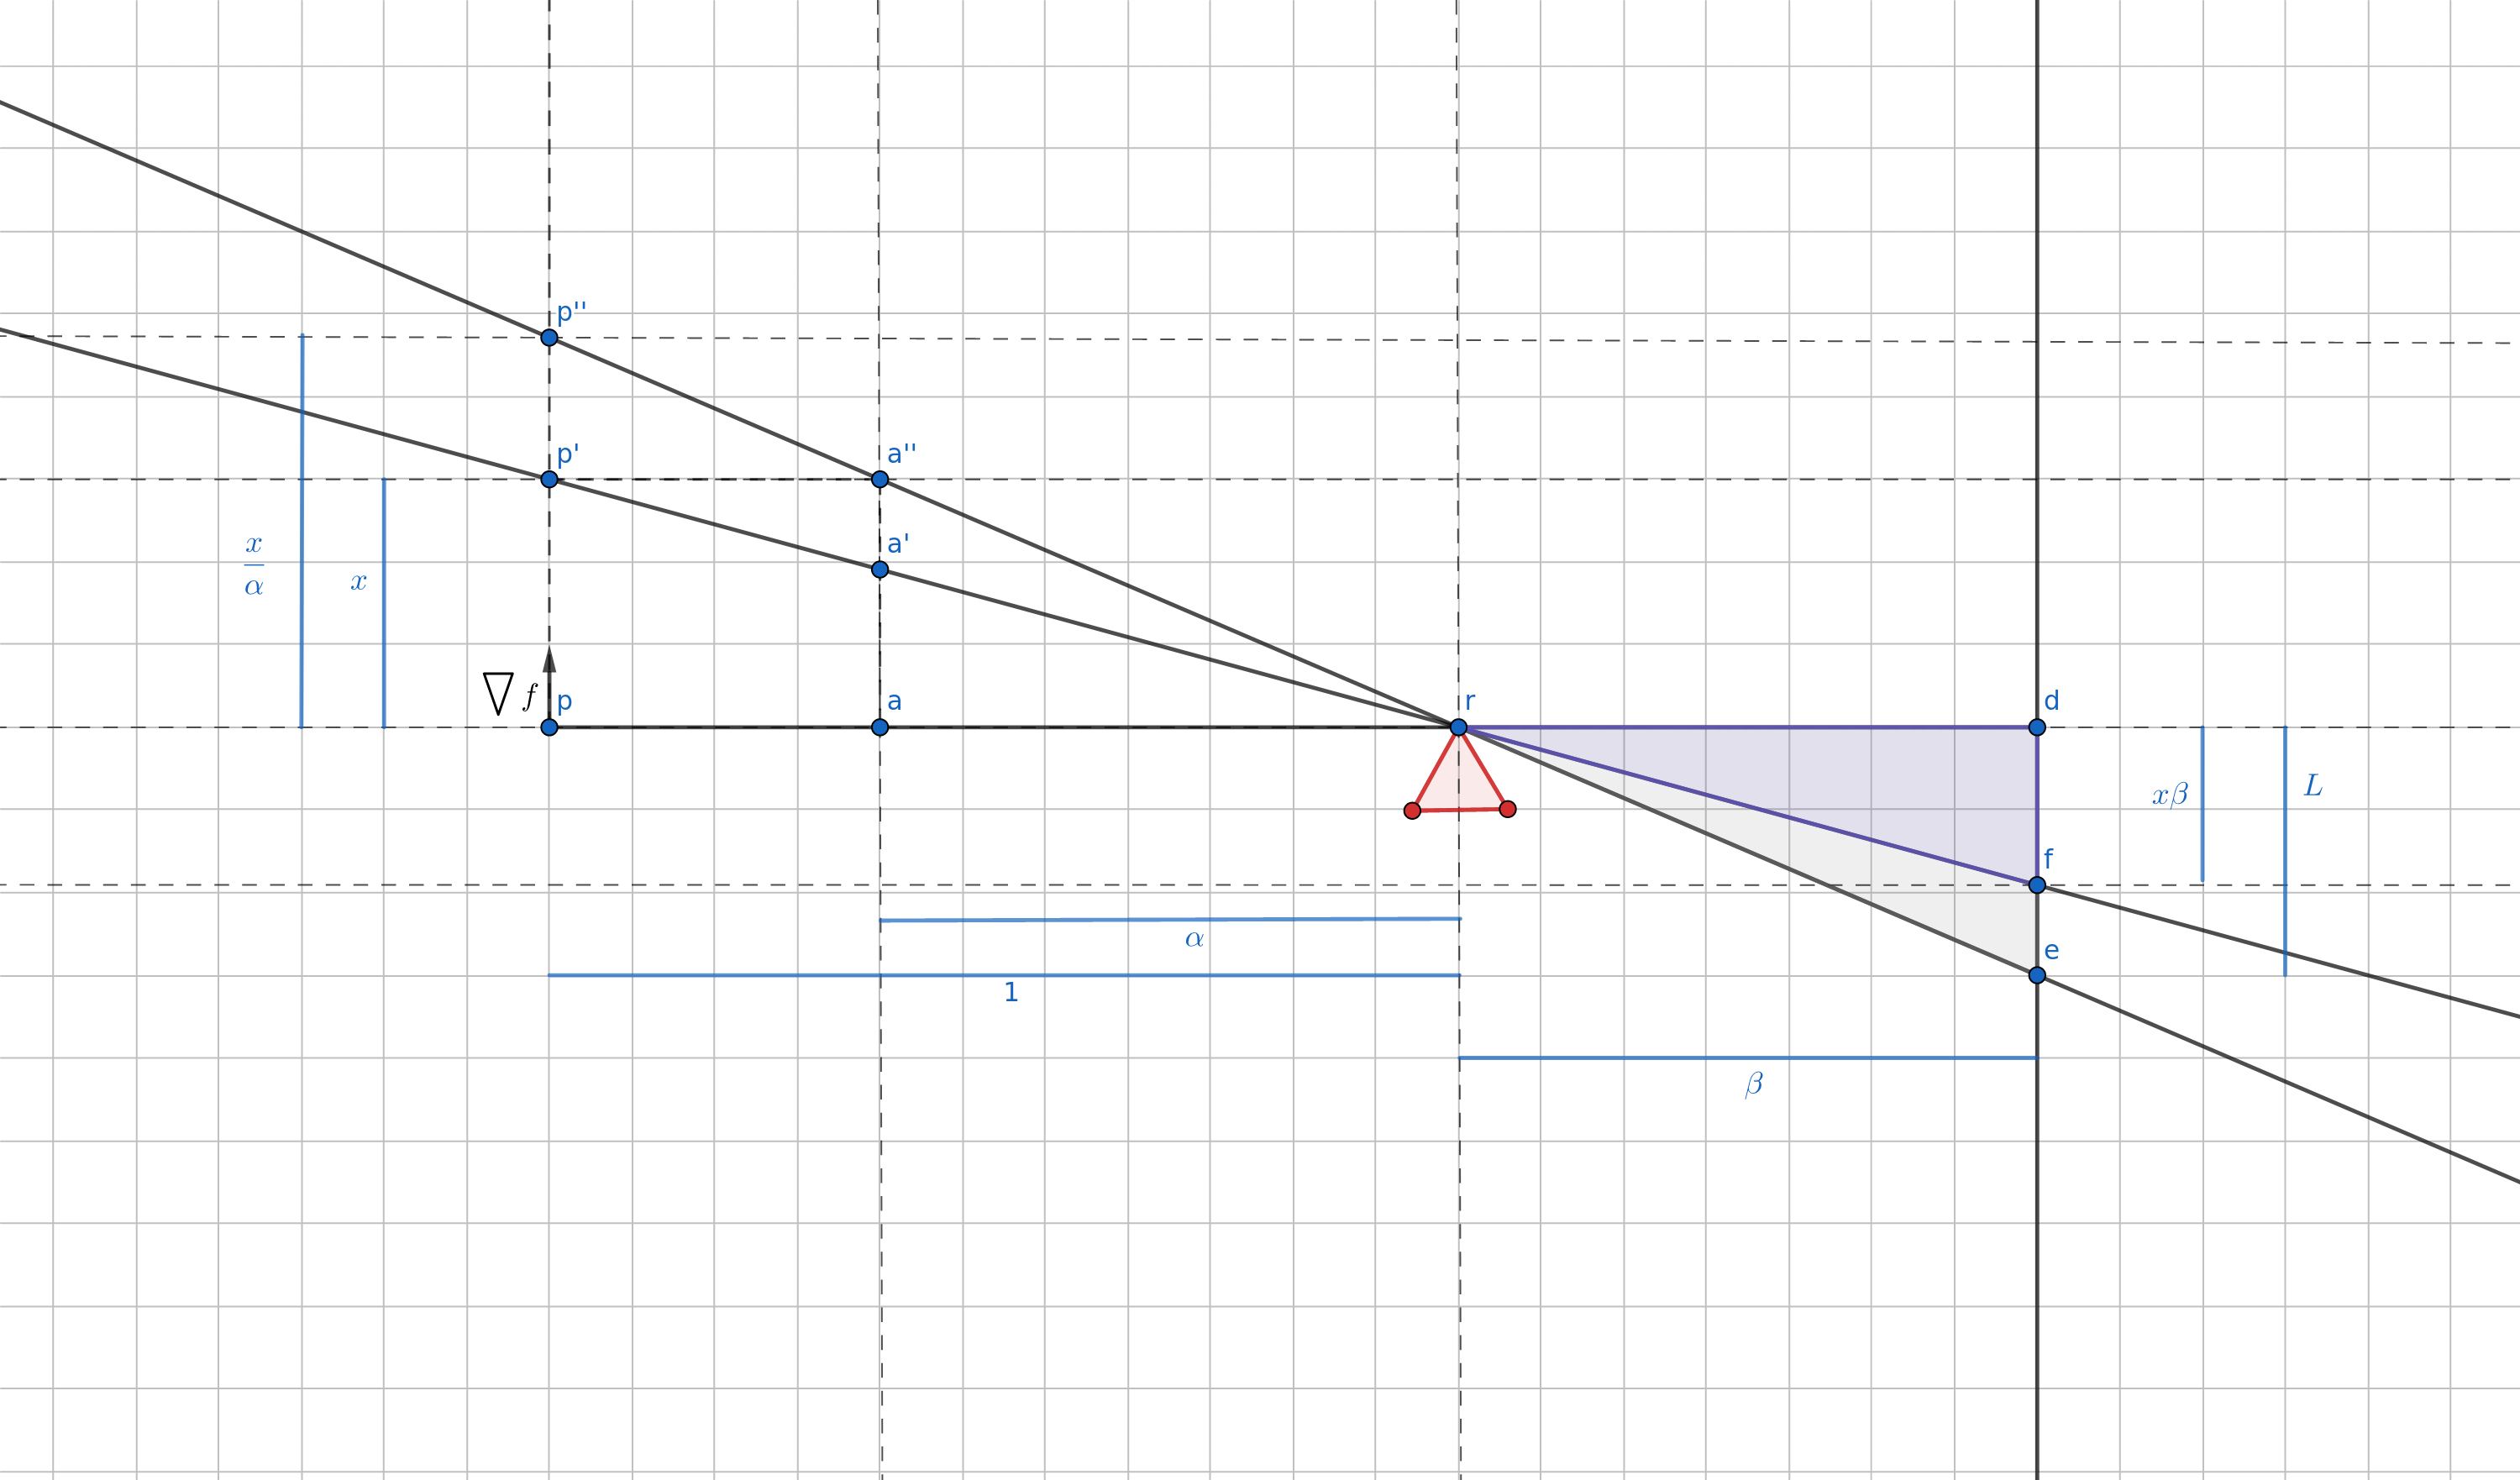
\includegraphics[width = 0.6\textwidth]{gradient.png}
    \caption{Illustrative example of applying gradient descent.}
    \label{fig:gradient_descent}
\end{figure}

\subsection{Thesis Goal}
This thesis will thus be an optimisation algorithm engineering paper. The main goal is to create and implement an algorithm that uses gradient descent to approximate the solution to the Art Gallery Problem. The explored research question will be whether the Art Gallery Problem can be efficiently solved using gradient descent. Additional to gradient descent, the algorithm will deploy different heuristics to address various shortcomings and edge-cases.
% As such, we expect to be able to provide convergence guarantees for the algorithm. 
The algorithm will be implemented in C ++ using the CGAL library (\url{https://www.cgal.org}).

This paper is organised as follows: Section \ref{sec:literature} offers an overview of existing work; Section \ref{sec:theory} explains how in theory gradient descent is used to solve the Art Gallery Problem and what heuristics we can make use of to improve the performance of our algorithm; Section \ref{sec:experiments} offers an overview of how well our algorithm performs in practice. Lastly, Section \ref{sec:problems} reveals issues this project has encountered.
% As such, preliminary research and its implementation is presented as preparation for the second phase of the thesis project. Section \ref{sec:literature} offers an existing literature overview. Next, Section \ref{sec:theory} describes the relevant theory in detail.
% As a preview, Section \ref{sec:experiments} shows some introductory algorithm implementations and their performance.
% Lastly, Section \ref{sec:thesis} presents the development plan for the second phase of the Master's Thesis project.

\subsection{Discussion}
As previously mentioned, this thesis focusses on implementing and evaluating a gradient descent algorithm to find a solution to the Art Gallery Problem. Indeed, this goal has been achieved for a few cases. 
Nonetheless, it is worth discussing the development process and the performance of the algorithm. Gradient descent is quite a straight-forward approach. However, its implementation in the context of the Art Gallery Problem is not. There were numerous edge-cases to be taken into account. For many of them, we created various hyperparameterised heuristics. Other heuristics (momentum) were created as an improvement to the shortcomings of the vanilla version of gradient descent.

The resulting program is sensitive to hyperparameter choices, polygon shapes and starting guard positions. For this reason, we only provide qualitative evaluations for the heuristics used to extend gradient descent. Namely, Section \ref{sec:experiments} discusses the added benefits of each of the heuristics used. The way this is done is by running the program with all heuristics but the one whose practicality we are discussing. In this way, we will assess its significance in its absence. The reason behind this experimental setup is that combinations of all heuristics are both verbose and unnecessary. Given that the program is still limited to a few number of examples, we cannot use extensive statistical tools to test its performance.
In this way, we provide a pragmatic overview to the usefulness of each of the heuristics and hyperparameters used. Namely, we analyse on what the type of polygons different heuristics and hyperparameter values provide concrete results.

Section \ref{sec:future} will further discuss about how the program could be improved in the future.



% - evaluation of what I did
%     - selection of heuristics that make sense (because their combination is too long)
% - "conclusion"

\subsection{Future Work}
\label{sec:future}
Currently, the program offers a state-of-the-art view about its practical possibilities.
In the future, it would be suitable to extend it with more robust functionalities.

One of the most crucial aspects of improvement for the program would be to solve the existing errors and bugs. As of now, the program crashes for specific input polygons (see Section \ref{sec:problems} for an extensive overview of its shortcomings). Another important element to consider would be to code it more efficiently. Some of the data structures used are naive and can be easily implemented in a smarter way. For this reason, the program does not scale well. 

Additionally, some features and heuristics are not complete. For example, the greedy initialisation of the guards' position is deterministic. In order to quantitatively assess the performance of the algorithm, a truly randomised greedy initialisation would be required for statistical significance.

Lastly, it would be worth exploring how the algorithm would benefit from a different implementation. Namely, using another programming language like Python (or CGAL Python bindings) and other geometry libraries which are better documented and more reliable to use.
% - improve the efficiency of the code
%     - can add a flag for guards whose gradient has been computed instead of copying the vector
% - find a more efficient way of coding to tackle the edge-cases
% - implement an expiry date for the reflex area
% - implement algorithm for love polygon - currently crashes 
% - init gradient is not randomised -> should do that for finding actually working starting positions
% - give an impression on the code improvement
